\documentclass{article}

% if you need to pass options to natbib, use, e.g.:
% \PassOptionsToPackage{numbers, compress}{natbib}
% before loading nips_2017
%
% to avoid loading the natbib package, add option nonatbib:
% \usepackage[nonatbib]{nips_2017}

\usepackage{nips_2017}

% to compile a camera-ready version, add the [final] option, e.g.:
% \usepackage[final]{nips_2017}

\usepackage[utf8]{inputenc} % allow utf-8 input
\usepackage[T1]{fontenc}    % use 8-bit T1 fonts
\usepackage{hyperref}       % hyperlinks
\usepackage{url}            % simple URL typesetting
\usepackage{booktabs}       % professional-quality tables
\usepackage{amsfonts}       % blackboard math symbols
\usepackage{nicefrac}       % compact symbols for 1/2, etc.
\usepackage{microtype}      % microtypography
\usepackage{wrapfig}
\usepackage{graphicx}


\title{Gradient Descent for Sharpe Ratio Optimization}

% The \author macro works with any number of authors. There are two
% commands used to separate the names and addresses of multiple
% authors: \And and \AND.
%
% Using \And between authors leaves it to LaTeX to determine where to
% break the lines. Using \AND forces a line break at that point. So,
% if LaTeX puts 3 of 4 authors names on the first line, and the last
% on the second line, try using \AND instead of \And before the third
% author name.

\author{
 Joseph Nunez\\
Seminar in Differential Geometry\\
Harvey Mudd College\\ 
March 7, 2018}

\begin{document}
% \nipsfinalcopy is no longer used

\maketitle


\abstract{A classical problem in portfolio management is the optimization of the Sharpe ratio: the ratio of a portfolio’s returns to its level of risk. We develop a Sharpe ratio optimization algorithm which uses gradient descent of the Kullback-Leibler divergence to determine the proportions with which to allocate a portfolio to optimize the Sharpe ratio. We backtest our algorithm on a universe of 25 stocks with data from Quandl.com, and we observed a 21.49\% increase in portfolio value over the last 150 trading days, a period during which the Dow Jones industrial Average increased by 15.80\%. This initial result is very promising, and invites further study, including extending the problem to include the possibility of going short in stocks as well as long.}

\section{Introduction}
A common goal of investors is to achieve the highest possible rate of return on invests while exposing themselves to as little risk as possible. When evaluating investments based on this paradigm, it is useful to consider the Sharpe ratio, which the ratio of an investment’s return (or expected return) over the risk associated with that investment. I will propose a strategy for maximizing the Sharpe ratio of a portfolio to be distributed across n assets using gradient descent. This strategy will rely upon conventional quantitative measures of risk and expected returns from finance and portfolio theory, then use geometric methods to determine the optimal portfolio configuration according to those measures.
The gradient descent algorithm we produce relies upon a number of approaches taken from portfolio theory about how to measure the expected return and risk of a portfolio of stocks. In particular, we will need to define what a portfolio is in the context of our algorithm, how we measure a portfolio’s expected returns, and how we determine the risk level of a portfolio. The proof of our algorithm also relies on results from information geometry, so some conclusions from information geometry will be included as well that will be discussed in this section as well.
\subsection{Portfolio Representation}
\begin{wrapfigure}{r}{0.3\textwidth}
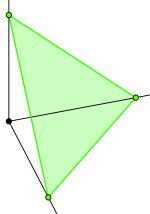
\includegraphics[scale=0.2]{simplex}
\caption{A simplex in R3 [8]}
\end{wrapfigure}
A portfolio of n stocks denoted $a_1 , \dots , a_n$ can be represented as a sequence of weights $\pi_1, \dots , \pi_n$, where
\begin{equation}
\sum_{i=1}^n \pi_i =1; \quad 0 \leq \pi_i \leq 1 \forall i.
\end{equation}
Each weight $\pi_i$ corresponds to the proportion of the portfolio allocated to $a_i$. The set of all points satisfying these constraints, points in $\mathbb{R}^n$ whose coordinates sum to 1 and are individually bounded by 0 and 1, is an $n$-dimensional simplex, a hyperplane of $\mathbb{R}^n$ with some
special properties. In particular, simplexes are a focus of information geometry. Therefore, we can use an $n$-dimensional simplex to represent all possible portfolios of $n$ stocks

\subsection{Portfolio Returns}
\begin{wrapfigure}{r}{0.3\textwidth}
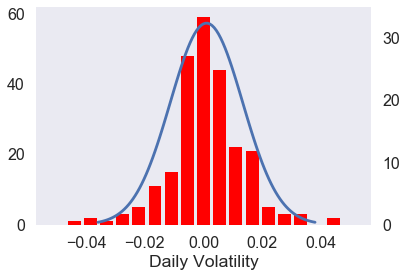
\includegraphics[scale=0.3]{aaplnormal}
\caption{The distribution of the log daily returns of AAPL overlaid with a normal distribution with matching standard deviation and mean}
\end{wrapfigure}
It has been empirically observed in the field of finance that asset prices follow a log normal distribution. That is, the logarithmic continuous growth rates of asset prices roughly fit a normal distribution, though in practice the distributions of returns tend to have thinner sides and fatter tails than normal distributions owing to the existence of news events such as earning reports that cause large, sudden shifts in asset prices. Figure 2 visually shows how well asset returns fits a normal distribution, in this case using the past year’s daily return for Apple stock.
To compute the log continuous growth rates for an asset,
we will look at the daily close of each asset $a_i$’s price (the
value of the asset at 4:00 PM ET, when markets close), divide it by the previous day's close, then take the logarithm
of that ratio. Once we have done so for every day in our
sample (we use one year’s worth of data for ever trading day), we take the mean, which gives us our expected daily return over the long run $\mu_i$. The standard deviation of the log returns gives us $\sigma_i$, which will act as our proxy for risk.
Once we have the expected return $\mu_i$ for each asset $a_i$ in our portfolio, the expected returns of the overall portfolio is simply a weighted sum of the returns of the individual assets
\begin{equation}
\mu_\pi = \sum_{i=1}^n \pi_i \mu_i
\end{equation}
The risk level of portfolio is slightly less straightforward, owing to the fact that the returns of different assets are correlated with one another. As such it is necessary to use the covariance between pairs of assets when calculating the risk of the portfolio overall. Let $R_i$ be the distribution of returns corresponding to asset ai. Using the statistical formula for the risk of correlated distributions, we get
\begin{equation}
 \sum_{i,j=1}^n \sigma_\pi^2 = \pi_i \pi_j Cov(R_i,R_j),
\end{equation}
where $Cov(Ri,Rj)$ is the covariance of the returns for assets $i$ and $j$ [1].


\section{Portfolio Return Distributions}
Using our expected return and risk measures, we see that every portfolio can be mapped to a normal distribution. It is therefore useful to have a measure of difference between normal distributions. We will use the Kullback-Leibler divergence, defined over continuous probability distributions as
\[D_KL(p,q) = \int_{-\infty}^\infty p(x) \log\frac{p(x)}{q(x)}\]
Let $p$ and $q$ be Gaussian distributions with respective means $\mu_1$ and $\mu_2$ and standard deviations $\sigma_1$ and $\sigma_2$. We wish to find a closed form for the $KL$-divergence. First, we can separate the logarithm to get
\[D_{KL}(p, q) = \int_{-\infty}^{\infty} p(x) \log p(x)dx − \int_{-\infty}^{\infty} p(x) \log q(x)dx\]
Recall that the equation of a Guassian is
p(x) log q(x)dx.
−∞
−∞
1 −(x−μ1)2
e 2σ2
p(x) =  
2πσ12 2
 ∞ p(x)
Figure 2: The distribution of the log daily returns of AAPL overlaid with a normal distribution with matching stan- dard deviation and mean.
 −∞
p(x)log q(x)dx.
   
Thus the first term becomes
 ∞
p(x) log  
1 −(x−μ1)2 2 e 2σ12
dx
   −∞ 2πσ1 Then the logarithm further simplifies to
1 2   ∞
(x − μ1)2 p(x) 2σ2 dx
2 log 2πσ1
This separates into three integrals when the square gets expanded
  p(x)x2dx −   p(x)2μ1xdx +   p(x)μ21dx 21 2σ12
The third integral becomes μ21 since Guassians have area 1. The first two integrals become the expectations of x2 and 2μ1x. Since variance of x is equal the expectation of x2 minus the square of the expectation of x, the expectation of x2 is equal to σ12 + μ21. The expectation of x is simply μ1. This yields
1log2πσ2+σ12+μ21−2μ21+μ21 =1log2πσ2+1 21 2σ12 222
  1
log 2πσ2
−∞ 1
      Which factors to become 1 (1 + log 2πσ2). 21
Similarly, the second term can be rewritten as
This separates into three integrals when the square gets expanded
1   p(x)x2dx −   p(x)2μ2xdx +   p(x)μ2dx 2 log 2πσ12 + 2σ2
The third integral becomes μ2 since Guassians have area 1. The first two integrals become the expectations of x2 and 2μ2x. Since variance of x is equal the expectation of x2 minus the square of the expectation of x, the expectation of x2 is equal to σ12 + μ21. The expectation of x is simply μ1. This yields
1log2πσ2+σ12+μ21−2μ1μ2+μ2 =1log2πσ2+σ12+(μ1−μ2)2 22 2σ2 22 2σ2
Combining these expressions, we get
1 2 σ 12 + ( μ 1 − μ 2 ) 2 1 2 2log2πσ2 + 2σ2 −2(1+log2πσ1)
  ∞ −∞
1 −(x−μ2)2 2 e 2σ2
2πσ2
−∞ 2
 dx   2  ∞ (x−μ2)2
p(x) log  
log 2πσ2 − p(x) 2σ2 dx
             We then combing the logarithms to get 2 log 2πσ12 σ 2
= 2 log σ12 = σ1 , which yields σ 12 + ( μ 1 − μ 2 ) 2 1
1 2πσ2 1 σ2 σ2
     2σ2 −2. (4) This will serve as the closed form to be used in the implementation of the algorithm [3].
KL(p,q)=logσ + 12
   3 Information Geometry
Information geometry is the study of the manifold of probability distributions, called the statistic manifold, or S, and was developed primarily by Shun-ichi Amari. Notably, when dealing with probability distributions with n disjoint outcomes, the set of all such distributions is an n-dimensional
3

simplex, since each outcome must have a probability between 0 and 1 and the cumulative probability of all outcomes must be 1.
In his 1992 paper ‘Information Geometry of Boltzmann Machines’, Amari proved that Boltmann machines, recurrent neural networks which learn to reproduce a probability distribution, will always converge to a global optimum approximation of the target distribution. Boltzmann machines have a set of connection weights which represent the probability of a certain node being 0 or 1. For a machine with n nodes, there are 2n possible outcomes, so the set of possible weights is a (2n − 1)-dimensional simplex. To find the best approximation of a target distribution within this space, a Boltzmann machine performs stochastic gradient descent of the KL-divergence between the distribution it is realizing and the target distribution. In proving that Boltzmann machines will always converge to the global best approximation, Amari demonstrated that there is a dually affine connection between the error surface of the KL-divergence over a finite-dimensional simplex [2].
In the context of gradient descent, the error surface is defined by the map
\[D : S \rightarrow R;\]
\[s  \mapsto D(p(s), y)\]
where $S$ is the space of possible weights, $D$ is a distance function, $s$ is a set of weights in $S$, $p(s)$ is the prediction generated based on the weights $s$, and $y$ is the target trying to being realized. Amari demonstrated that the error surface is smooth and lacks local minima when it the weight space is a finite dimensional simplex. Therefore, by traveling down the gradient of the error surface, an algorithm is guaranteed to reach the global minimum of the error surface.
Therefore, because our weight space for our portfolio configurations is a finite-dimensional simplex, we want to construct our problem in the context of minimizing the $KL$-divergence between the distribution of the log returns of our portfolio and some target distribution. If we do so, Amari’s conclusions allow us to guarantee that using gradient descent will find the optimal portfolio configuration.
\section{Methods} 
The methods section consists of both the gradient descent algorithm itself and the methods used to backtest the algorithm’s performance. The gradient descent algorithm is an alteration of stochastic gradient descent algorithms owing to the fact that rather than having a large set of sample inputs and target outputs, we instead have one target distribution and a single set of input stocks. As a result, rather than stochastically estimating the gradient, we actually compute the gradient with respect to the portfolio weights. My backtesting approach rather simply applies the algorithm every day to compute new weights, invests based on that, and records the resulting change in portfolio value at the end of each day.
4.1 Gradient Descent Algorithm
To perform gradient descent over an error surface, at each point, we need to calculate the gradient with respect to the weights, then take a small step in the direction of most negative gradient. We do this until the error stops changing with successive steps, indicating a gradient of the zero vector, which indicates a minimum. Since the error surface has no global minima, this minimum must represent the portfolio weights with the least error.
To implement this algorithm, we must compute the gradient of the KL-divergence with respect to each portfolio weight πi. Let p be the distribution of log returns generated according to the portfolio weights and let q be the target distribution. Let μ1 and μ2 be the respective means μ1 and μ2 and σ1 and σ2 be the respective standard deviations of p and q. Then we have
∂ ∂ σ 2 σ 12 + ( μ 1 − μ 2 ) 2 1 ∂πDKL(p,q)=∂πlogσ + 2σ2 −2.
ii12
Now take our expressions from section 1.2 for the return and risk of a portfolio, which are given by
n
μπ = πiμi, i=1
     4

n
σπ2 =   πiπjCov(Ri,Rj),
i,j =1
and plug them into the divergence formula. To avoid confusion, we’ll now use σ and μ for the
standard deviation and mean of the target distribution:
  n
∂ DKL(p,q)= ∂ (logσ−log   πiπjCov(Ri,Rj) ∂πi ∂πi  
i,j =1
 ni,j=1 πiπjCov(Ri,Rj)+( nj=1 πjμj −μ)2 1
+ 2σ2 − 2)
Now we’ll compute the partial derivative of each term. Note that σ and μ are constant with respect to
πi since the target does not change depending on the weights. The log σ and 1 are constants, so they
      become zero in the partial derivative. The other log term becomes
  n 1 ∂  
2
 −  n π π Cov(R ,R ) ∂πi   πiπjCov(Ri,Rj) i,j=1 i j i j i,j=1
   n
 
i,j=1πiπjCov(Ri,Rj)2 i,j=1πiπjCov(Ri,Rj) i i,j=1  nj=1,j̸=i πjCov(Ri,Rj)+2πi
11∂ = −  n   n ∂π
πiπjCov(Ri,Rj)
     = − 2 ni,j=1 πiπjCov(Ri,Rj) .
Notice that the 2πi is a result of there being a single π12 in the summation and Cov(Ri, Ri) = 1. The
next term should be split up into two fractions:
 ni,j=1 πiπjCov(Ri,Rj) + ( nj=1 πjμj −μ)2 2σ2 2σ2
The first fraction gets treated just like the previous summation and becomes
    The second fraction becomes
 nj=1,j̸=i πjCov(Ri,Rj)+2πi. 2σ2
2( nj=1πjμj−μ)∂  n
2σ2 ∂π ( πjμj −μ)
i j=1
= μi( nj=1 πjμj − μ). σ2
   Taken all together, we get that the partial derivative of the Kullback-Leibler divergence with respect to πi is
 nj=1,j̸=i πjCov(Ri,Rj)+2πi  nj=1,j̸=i πjCov(Ri,Rj)+2πi μi( nj=1 πjμj −μ) − 2 ni,j=1 πiπjCov(Ri,Rj) + 2σ2 + σ2
It’s straightforward to precompute the covariance matrix and expected returns for all of the assets’ returns ahead of time, so everything in this expression is in terms of readily available information, so this can be computed easily inside of an algorithm.
To perform gradient descent according to this rule, during each update step (also called training epoch), the weights are updated according to the following rule:
πt=k+1 = πt=k − ε∇[DKL(p(πt=k), q)]DKL(p(πt=k), q),
Where πt=k is the portfolio weight vector after k update iterations, p is the function that turns the portfolio weights into a distribution of returns, q is target distribution, DKL is the Kullback-Leibler divergence, and ∇ is the gradient operator with respect to all of the πis.
   5

We will also use a variable learning rate, which is a mechanism that gradient descent algorithms use to help them converge faster. The variable learning rate strategy we used is to increase ε by a factor of 1.05 whenever the most recent update caused the error to decrease and to decrease ε by a factor of 0.7 whenever the most recent update caused the error to increase by a factor of 1.04 or greater. My implementation of the algorithm used 800 training epochs and an initial learning rate of ε = 0.001. These values were chosen through trial and error to get the algorithm to quickly and consistently converge.
Up to this point, we have discussed the gradient descent algorithm in terms of approaching a target distribution rather than optimizing the Sharpe ratio of the portfolio. Since gradient descent requires a target to approach, this is a necessity, but it means that we must choose the target distribution such that minimizing the divergence from the target distribution maximizes the Sharpe ratio. Fortunately, this choice is relatively straightforward: choose a distribution with an unachievably high Sharpe ratio, but also close enough to the achievable distributions that the divergence is meaningfully different for different achievable distributions. As the algorithm seeks to get closer to this distribution, the portfolio’s Sharpe ratio will increase. For our target’s growth rate, we choose the maximum growth rate among the individual stocks because the portfolio cannot grow faster than its fastest-growing element. For our target risk level, we don’t know what the true minimum risk is since that depends upon the covariances, but we know that we can minimize the πiπj component of each term in the summation by evenly distributing our portfolio across all of the assets. To be extra cautious and ensure we don’t overestimate the minimum risk, we’ll also divide this risk by a factor of 10. Now we have μ and σ for our target distribution.
4.2 Backtesting
I implemented by backtesting script in Python 3 in a Juptyer Notebook. Unfortunately, I cannot make a functioning version of this code publicly available, as it requires a Quandl API key to run, and Quandl’s terms of service forbid sharing one’s API key. The stocks I considered investing in were 25 stocks chosen from the Dow Jones Industrial Average (DJIA). The five DJIA stocks I did not consider were excluded because my data source, Quandl.com, did not have enough of their historical pricing data freely available in order for me to include them in my testing1.
For each of the past 150 trading days\footnote{The stocks I excluded were 3M (MMM), Apple (AAPL), DowDuPont (DWDP), Intel (INTC), and Travelers Companies (TRV).}$^,$\footnote{Trading days are Mondays through Fridays excluding holidays. 3The last trading day I used in my testing was February 28, 2018.}, I ran the gradient descent algorithm on the previous year’s worth of data (251 trading days) to obtain the portfolio weights with the best Sharpe ratio.
I then calculated the returns that a portfolio with the determined weights would have had on that day and applied that rate of return to a portfolio with an initial value of \$10,000. For the sake of comparison, I also tracked the performance of the Dow Jones Industrial Average over that time period as a baseline, and applied that growth rate to a portfolio with an initial value of \$10,000.
\section{Results}
In Figure 3 on the following page, the orange line represents the performance of \$10,000 invested in a DJIA index or mutual fund, and the blue line represents the performance of \$10,000 invested according to the algorithm.
Over the course of 150 trading days, the gradient descent algorithm resulted in a growth rate of 21.49\% compared with a growth of only 15.80\% for the market as a whole. Interestingly, the period between trading days 130 and 140 saw a rapid decline in the investments made by our algorithm, though this is unsurprising as it coincided with a very sharp decline in the stock market (including the single largest point loss in the DJIA in a single day). The particular reasons for this crash are still unclear, but many speculate that it was caused by broad fears that stocks in general were overpriced, which lead to selling off stocks across all sectors, which meant that even historically uncorrelated stocks behaved similarly. Our risk estimates considered such an event highly unlikely based on our covariance values, so the portfolio was poorly configured for such an event. However, our portfolio


 Figure 3: 150 trading days backtest of algorithm versus DJIA baseline
did not underperform the market during this time, indicating that our algorithm does not overexpose us to these events relative to the market as a whole.
More importantly, during the low volatility period that marks the beginning of the graph, we see that our algorithms gradually outperforms the market, as our optimization gives us a slight edge over the market when the stocks are performing as expected. When this is coupled with the fact that our algorithm does not face greater risk over the market, we see that our algorithm will gradually outpace the market over time.
6 Acknowledgments
Thank you to professors Gu, Evans, and Sweedyk for courses in which I developed the background knowledge of information geometry, gradient descent algorithms, and financial economics necessary to complete this project. Parts of the code I used during this project were adapted from code developed during these courses.
7 Future Work
This algorithm demonstrates the gradient descent along an error surface generated by the Kullback- Leibler divergence is a promising approach for tackling problems in portfolio theory. There are several directions in which to expand this algorithm.
First, we could expand the weight space beyond 0 and 1 to allow for the potential to go short in an asset and use the capital from the short sale to go extra long in another asset. This approach would require altering the function that converts the weights to a portfolio and calculates its distance from the target distribution. We would need to prove this new function to still produce an error surface with no local minima, and to recompute the gradient to account for this change.
Another extension would be to study the rebalancing frequency. Out of convenience with respect to data availability, I used daily returns, hence optimizing the Sharpe ratio over a 1-day horizon, so I
7

rebalanced daily. It’s quite possible that this is not the optimal frequency with respect to long-term growth, and insight into this problem could be found in Wong’s thesis, which focused on rebalancing frequency [1].
There is also the possibility of exploring different risk metrics to use; I recently heard of a type of probability distribution called a Slash distribution, which has similar features to a normal distribution, but features the narrower sides and fatter tails which have been empirically observed in asset log growth rates.

\section*{References}
[1] Wong, T. 2016, ’Geometry and Optimization of Relative Arbitrage’, PhD Thesis, University of Michigan, Ann Arbor MI.
[2] Amari, S., Kurata, K., Nagaoka, H. 1992, ’Information Geometry of Boltzmann Machines’, IEEE Transac- tions on Neural Networks, 260-271.
[3] ‘KL divergence between two univariate Gaussians’, Stats.stackexchange.com, \url{https://stats. stackexchange.com/questions/7440/kl-divergence-between-two-univariate-gaussians}
[4] ‘NumPy Reference — NumPy v1.14 Manual’, Docs.scipy.org, \url{https://docs.scipy.org/doc/numpy/ reference/}
[5] ‘Matplotlib 2.2.0 documentation’, Matplotlib.org, \url{https://matplotlib.org/#documentation}
Data Sources:
[6] ‘Quandl’, Quandl.com, \url{https://www.quandl.com/}
[7] ‘∧DJI Historical Prices | Dow Jones Industrial Average Stock - Yahoo Finance’, Finance.yahoo.com, \url{https://finance.yahoo.com/quote/%5EDJI/history?p=%5EDJI}
Image Sources:
[8] ‘Simplex’, Wikipedia.org, \url{https://en.wikipedia.org/wiki/Simplex}


\end{document}
